\documentclass[
    11pt, % Set the default font size, options include: 8pt, 9pt, 10pt, 11pt, 12pt, 14pt, 17pt, 20pt
    %
    aspectratio=169, % Uncomment to set the aspect ratio to a 16:9 ratio which matches the aspect ratio of 1080p and 4K screens and projectors
]{beamer}

\graphicspath{{Images/}{./}} % Specifies where to look for included images (trailing slash required)
\usepackage{booktabs} % Allows the use of \toprule, \midrule and \bottomrule for better rules in tables

%\usepackage{appendixnumberbeamer} %If you want a separate slide counter for your appendix

%%% Customize Theme %%%%%%%%%%%%%%%%%%%%%%
\usetheme{Madrid} % You can use other themes too, but this changes many things. I've found Madrid to be the best for this color scheme

%fg = font color
%bg = background color

% ! WARNING ! : Many colors are linked to multiple attributes, so changing one color can have unexpected changes!

% If you want to tweak the shading of colors, tweak the below 2 lines:
\definecolor{myBlue}{RGB}{20, 20, 255}
\definecolor{myTeal}{RGB}{150, 0, 0}

% Bottom right hand color
\setbeamercolor*{structure}{bg=myBlue!20,fg=myBlue!90}

\setbeamercolor*{palette primary}{use=structure,fg=white,bg=structure.fg} %?
\setbeamercolor*{palette secondary}{use=structure,fg=myBlue,bg=white}
    %bottom left of footer & bar between title & top bubbles
\setbeamercolor*{palette tertiary}{use=structure,fg=white,bg=myBlue}

\setbeamercolor{frametitle}{bg=myBlue!85,fg=white} %title of each slide

\setbeamercolor*{titlelike}{parent=palette primary} %?
%\setbeamercolor{titlelike}{parent=palette primary,fg=structure.fg!50!myBlue}

%for miniframe (very top) AND center footer
\setbeamercolor{section in head/foot}{fg=myTeal, bg=white}

%%% Specific Colors %%%
\setbeamercolor{item projected}{bg=myTeal}
\setbeamertemplate{enumerate items}{bg=myTeal}

\setbeamercolor{itemize item}{fg=myTeal}
\setbeamercolor{itemize subitem}{fg=myTeal}

\setbeamercolor{button}{bg=myTeal}

%%% Edits ONLY the TOC slide %%%
\setbeamercolor{section in toc}{fg=black}
\setbeamercolor{subsection in toc}{fg=black}

%%% Block Colors %%%
% Standard block %
    \setbeamercolor{block title}{bg=myTeal, fg=white}
    \setbeamercolor{block body}{bg=myTeal!20}

% Alerted block % If you want to customize it's color
    %\setbeamercolor{block title alerted}{bg=cyan, fg=white}
    %\setbeamercolor{block body alerted}{bg=cyan!10}

% Example block % If you want to customize it's color
    %\setbeamercolor{block title example}{bg=cyan, fg=white}
    %\setbeamercolor{block body example}{bg=cyan!10}

%---------------------------------------------------------
%	SELECT FONT THEME & FONTS
%---------------------------------------------------------
\usefonttheme{professionalfonts}
\usepackage{iftex}
\ifPDFTeX
  \usepackage[T1]{fontenc}
  \usepackage{newtxtext}
  \usepackage{newtxmath}
\else
  \usepackage{fontspec}
  \setmainfont{Times New Roman}
  \setsansfont{Times New Roman}
  \setmonofont{Courier New}
\fi
% Added math + TikZ
\usepackage{amsmath}
\usepackage{tikz}

\tikzset{>=latex} % for LaTeX arrow head
\colorlet{myred}{red!80!black}
\colorlet{myblue}{blue!80!black}
\colorlet{mygreen}{green!60!black}
\colorlet{mydarkred}{myred!40!black}
\colorlet{mydarkblue}{myblue!40!black}
\colorlet{mydarkgreen}{mygreen!40!black}
\colorlet{myorange}{orange!80!black}
\colorlet{myviolet}{blue!50!red!60}
\tikzstyle{node}=[very thick,circle,draw=myblue,minimum size=22,inner sep=0.5,outer sep=0.6]
\tikzstyle{connect}=[->,thick,mydarkblue,shorten >=1]
\tikzset{ % node styles, numbered for easy mapping with \nstyle
  node 1/.style={node,mydarkgreen,draw=mygreen,fill=mygreen!25},
  node 2/.style={node,mydarkblue,draw=myblue,fill=myblue!20},
  node 3/.style={node,mydarkred,draw=myred,fill=myred!20},
}
\def\nstyle{int(\lay<\Nnodlen?min(2,\lay):3)} % map layer number onto 1, 2, or 3

\usetikzlibrary{arrows.meta,shadows,positioning}
\usepackage{listofitems} 
\usetikzlibrary{calc}
\usetikzlibrary{fit, positioning, shapes.geometric}
\tikzset{
	frame/.style={
		rectangle, draw,
		text width=6em, text centered,
		minimum height=4em,drop shadow,fill=white,
		rounded corners,
	},
	line/.style={
		draw, -{Latex},rounded corners=3mm,
	}
}
\usetikzlibrary{arrows.meta,positioning,calc,decorations.pathmorphing}
\usepackage{subcaption} % added for side-by-side subfigures
\pgfmathsetmacro{\r}{0.8}
\pgfmathsetmacro{\Phi}{-160}
\pgfmathsetmacro{\Theta}{-90}
\usepackage{fontawesome5}
\usepackage{float}
\usepackage{amsmath}
\usepackage{physics}
\usepackage{algorithm, algorithmic}
\usetikzlibrary{arrows.meta,positioning,calc,decorations.pathmorphing}

\useinnertheme{circles}

%---------------------------------------------------------
%	SELECT OUTER THEME
%---------------------------------------------------------
% Outer themes change the overall layout of slides, such as: header and footer lines, sidebars and slide titles. Uncomment each theme in turn to see what changes it makes to your presentation.

%\useoutertheme{default}
%
\useoutertheme{miniframes}

% \useoutertheme{infolines}
% \useoutertheme{smoothbars}
% \useoutertheme{sidebar}
% \useoutertheme{split}
% \useoutertheme{shadow}
% \useoutertheme{tree}
% \useoutertheme{smoothtree}

%---------------------------------------------------------
%	PRESENTATION INFORMATION
%---------------------------------------------------------

\title[Multi-Agent RL for Spacecraft Guidance]{Robust Reinforcement Learning Differential Game Guidance in Low-Thrust, Multi-Body Dynamical Environments}
\subtitle{A Zero-Sum Reinforcement Learning Approach in Three-Body Dynamics}
\author[Ali Baniasad]{Ali Baniasad \\ \smallskip Supervisor: Dr. Nobahari}

\institute[]{Department of Aerospace Engineering \\ \smallskip Sharif University of Technology}
\date[\today]

\logo{
\includegraphics[width=1.cm]{sharif_logo.png}}

%---------------------------------------------------------
%---------------------------------------------------------
%---------------------------------------------------------
\begin{document}

%---------------------------------------------------------
%	TITLE SLIDE
%---------------------------------------------------------
\section{}
\begin{frame}
	\titlepage % Output the title slide, automatically created using the text entered in the PRESENTATION INFORMATION block above

\end{frame}

%---------------------------------------------------------
%	TABLE OF CONTENTS SLIDE
%---------------------------------------------------------

\begin{frame}
	\frametitle{Outline}
	\tableofcontents
\end{frame}

% --- Chapters added from report ---
% %\section{
%    یادگیری تقویتی
%    }
%

%--------------------------------------------------------------------
\section{یادگیری تقویتی}\label{sec:rl}

یادگیری تقویتی\LTRfootnote{Reinforcement Learning (RL)}
 شاخه‌ای از یادگیریِ ماشین است که در آن توالیِ اقدام‌ها $\boldsymbol{a}_t\in\mathcal{A}$ به‌گونه‌ای انتخاب می‌شود که بازدهِ تجمعیِ آینده بیشینه شود. یک فرایندِ تصمیم‌گیریِ مارکوف\LTRfootnote{Markov Decision Process (MDP)}
  به‌صورت $\langle\mathcal{S},\mathcal{A},p,r,\gamma\rangle$ تعریف می‌شود که در آن:
\begin{itemize}
	\item $\mathcal{S}$:
	 مجموعه‌ی حالات،
	\item $p(\boldsymbol{s}'|\boldsymbol{s},\boldsymbol{a})$:
	 دینامیکِ انتقال،
	\item $r(s,\boldsymbol{a})$:
	 پاداشِ آنی،
	\item $\gamma\in[0,1)$:
	 ضریبِ تنزیل.
\end{itemize}
\noindent
سیاست\LTRfootnote{Policy}
 $\pi(a|s)$ به‌عنوان احتمالِ انتخابِ اقدامِ $\boldsymbol{a}$ در وضعیتِ $\boldsymbol{s}$ بیان می‌شود. هدف، بیشینه‌سازیِ برگشت\LTRfootnote{Return}
 است:
 \begin{equation}
 	G_t=\sum_{k=0}^{\infty}\gamma^k r_{t+k}
 \end{equation}
 
 روش‌های \lr{RL} معمولاً در دو دسته‌ی {ارزش‌محور} (مانند \lr{Q-learning} و \lr{DQN}) و {سیاست‌محور} (مانند \lr{Reinforce}) جای می‌گیرند؛ ترکیبِ این دو به چارچوبِ \lr{Actor–Critic} منتهی می‌شود که در آن، یک بازیگر (\lr{Actor}) سیاست را به‌روزرسانی می‌کند و یک منتقد (\lr{Critic}) ارزش یا \lr{Q} برآورد می‌شود
  \cite{SuttonBarto2018}.

در حضورِ فضاهای پیوسته‌ی حالت–عمل، الگوریتم‌های  \lr{DDPG}، \lr{TD3}، \lr{SAC} و \lr{PPO} با تکیه بر شبکه‌های عصبی به‌عنوان تقریب‌گر توابع، کاراییِ بالایی نشان داده‌اند. در این پژوهش، خانواده‌ی \lr{Actor–Critic} به‌عنوان پایه‌ی توسعه‌ی کنترل‌کننده پیشنهاد شده‌ است و در ادامه، به نسخه‌ی چندعاملیِ آن در بخش~\ref{sec:marl} پیوند داده می‌شود.

% \chapter{یادگیری تقویتی چند عاملی}
کاربردهای پیچیده در یادگیری تقویتی نیازمند اضافه کردن چندین عامل\LTRfootnote{Multi-Agent} برای انجام همزمان وظایف مختلف هستند.
با این حال، افزایش تعداد عامل‌ها چالش‌هایی در مدیریت تعاملات میان آن‌ها به همراه دارد.
در این فصل، بر اساس مسئله بهینه‌سازی برای هر عامل، مفهوم تعادل\LTRfootnote{Equilibrium} معرفی شده تا رفتارهای توزیعی چندعاملی را تنظیم کند.
رابطه رقابت میان عامل‌ها در سناریوهای مختلف تحلیل شده و آن‌ها با الگوریتم‌های معمول یادگیری تقویتی چندعاملی ترکیب شده‌اند. بر اساس انواع تعاملات، یک چارچوب نظریه بازی برای مدل‌سازی عمومی در سناریوهای چندعاملی استفاده شده است. با تحلیل بهینه‌سازی و وضعیت تعادل برای هر بخش از چارچوب، سیاست بهینه یادگیری تقویتی چندعاملی برای هر عامل بررسی شده است.




  \section{تعاریف و مفاهیم اساسی }
یادگیری تقویتی چندعاملی\LTRfootnote{Multi-Agent Reinforcement Learning (MARL)} به بررسی چگونگی یادگیری و تصمیم‌گیری چندین عامل مستقل در یک محیط مشترک پرداخته می‌شود. برای تحلیل دقیق و درک بهتر این حوزه، اجزای اصلی آن شامل عامل، سیاست و مطلوبیت\LTRfootnote{Utility} در نظر گرفته می‌شوند که در ادامه به صورت مختصر و منسجم تشریح می‌گردند.

\begin{itemize}
	\item عامل: یک موجودیت مستقل به عنوان عامل تعریف می‌شود که به صورت خودمختار با محیط تعامل کرده و بر اساس مشاهدات رفتار سایر عامل‌ها، سیاست‌هایش انتخاب می‌گردند تا سود حداکثر یا ضرر حداقل حاصل شود. در سناریوهای مورد بررسی، چندین عامل به صورت مستقل عمل می‌کنند؛ اما اگر تعداد عامل‌ها به یک کاهش یابد، \lr{MARL} به یادگیری تقویتی معمولی تبدیل می‌شود.
	
	\item سیاست: برای هر عامل در \lr{MARL}، سیاستی خاص در نظر گرفته می‌شود که به عنوان روشی برای انتخاب اقدامات بر اساس وضعیت محیط و رفتار سایر عامل‌ها تعریف می‌گردد. این سیاست‌ها با هدف به حداکثر رساندن سود و به حداقل رساندن هزینه طراحی شده و تحت تأثیر محیط و سیاست‌های دیگر عامل‌ها قرار می‌گیرند.
	
	\item مطلوبیت: مطلوبیت
	هر عامل بر اساس نیازها و وابستگی‌هایش به محیط و سایر عامل‌ها تعریف شده و به صورت سود منهای هزینه، با توجه به اهداف مختلف محاسبه می‌شود. در سناریوهای چندعاملی، از طریق یادگیری از محیط و تعامل با دیگران، مطلوبیت هر عامل بهینه می‌گردد.
\end{itemize}

در این چارچوب، برای هر عامل در \lr{MARL} تابع مطلوبیت خاصی در نظر گرفته شده و بر اساس مشاهدات و تجربیات حاصل از تعاملات، یادگیری سیاست به صورت مستقل انجام می‌شود تا ارزش مطلوبیت به حداکثر برسد، بدون اینکه مستقیماً به مطلوبیت سایر عامل‌ها توجه شود. این فرآیند ممکن است به رقابت یا همکاری میان عامل‌ها منجر گردد.
 با توجه به پیچیدگی تعاملات میان چندین عامل، تحلیل نظریه بازی‌ها به عنوان ابزاری مؤثر برای تصمیم‌گیری در این حوزه به کار گرفته می‌شود. بسته به سناریوهای مختلف، این بازی‌ها در دسته‌بندی‌های متفاوتی قرار داده شده که در بخش‌های بعدی بررسی خواهند شد.

  % \section{اهمیت یادگیری تقویتی چندعاملی}

یادگیری تقویتی چندعاملی به دلیل قابلیت‌های بالقوه‌اش در مدل‌سازی و حل مسائل پیچیده و پویا، اهمیت زیادی در حوزه‌های مختلف علمی و صنعتی دارد. در این بخش، به بررسی اهمیت \lr{MARL} در زمینه‌های مختلف پرداخته و نقش آن را در توسعه سیستم‌های هوشمند متعدد بررسی می‌کنیم.

\subsubsection{مدل‌سازی سیستم‌های پیچیده و پویا}
یکی از دلایل اصلی اهمیت \lr{MARL}، توانایی آن در مدل‌سازی سیستم‌های پیچیده و پویا است. در بسیاری از کاربردهای واقعی، سیستم‌ها شامل چندین عامل هستند که به صورت همزمان و مستقل به تعامل می‌پردازند. به عنوان مثال، در شبکه‌های ترافیکی، هر خودرو می‌تواند به عنوان یک عامل مستقل عمل کند که نیاز به هماهنگی و تعامل با سایر خودروها برای بهینه‌سازی جریان ترافیک دارد. \lr{MARL} با فراهم کردن چارچوبی برای تعامل و یادگیری میان این عوامل، امکان بهبود کارایی و کاهش ترافیک را فراهم می‌کند.

\subsubsection{کاربرد در رباتیک چندعاملی}
در حوزه رباتیک، سیستم‌های چندعاملی می‌توانند برای انجام وظایف پیچیده‌ای مانند جست‌وجو و نجات، حمل و نقل مواد، و عملیات هماهنگ در محیط‌های غیرقابل پیش‌بینی مورد استفاده قرار گیرند. به عنوان مثال، گروهی از ربات‌های پرنده (دُرون‌ها) می‌توانند با همکاری و تبادل اطلاعات، منطقه‌ای وسیع را برای شناسایی اهداف نظارت کنند یا به سرعت به تغییرات محیطی واکنش نشان دهند. \lr{MARL} در این زمینه بهبود هماهنگی میان ربات‌ها و افزایش کارایی عملیات‌های چندعاملی را ممکن می‌سازد.

\subsubsection{مدیریت منابع در شبکه‌های ارتباطی}
شبکه‌های ارتباطی مدرن نیازمند مدیریت بهینه منابع مانند پهنای باند، انرژی و ظرفیت ذخیره‌سازی هستند. در این راستا، \lr{MARL} می‌تواند به عنوان یک ابزار قدرتمند برای تخصیص بهینه منابع به عوامل مختلف شبکه عمل کند. به عنوان مثال، در شبکه‌های بی‌سیم، هر دستگاه کاربر می‌تواند به عنوان یک عامل مستقل عمل کرده و با یادگیری و تعامل با سایر دستگاه‌ها، نحوه بهینه‌سازی مصرف انرژی و پهنای باند را پیدا کند. این امر منجر به افزایش کارایی شبکه و کاهش هزینه‌های عملیاتی می‌شود.

\subsubsection{توسعه الگوریتم‌های پیشرفته‌تر و قابل اعتمادتر}
یکی دیگر از جنبه‌های مهم \lr{MARL}، فهم و تحلیل تعاملات میان عوامل مختلف است که می‌تواند به توسعه الگوریتم‌های پیشرفته‌تر و قابل اعتمادتر منجر شود. با مطالعه رفتارها و استراتژی‌های مختلف در محیط‌های چندعاملی، پژوهشگران قادر به طراحی الگوریتم‌هایی می‌شوند که نه تنها بهینه عمل می‌کنند بلکه مقاومت بالایی در برابر تغییرات محیطی و رفتارهای غیرمنتظره دارند. این الگوریتم‌ها می‌توانند در شرایط متنوع و پیچیده‌تر به خوبی عمل کنند و از خطاها و ناهنجاری‌های احتمالی جلوگیری نمایند.

\subsubsection{کاربرد در بازی‌های چندعاملی و شبیه‌سازی‌های اقتصادی}
بازی‌های چندعاملی و شبیه‌سازی‌های اقتصادی از دیگر حوزه‌هایی هستند که به شدت از \lr{MARL} بهره‌مند می‌شوند. در بازی‌های استراتژیک چند نفره، \lr{MARL} می‌تواند به بازیگران کمک کند تا استراتژی‌های بهینه‌ای برای رقابت و همکاری با یکدیگر توسعه دهند. همچنین، در شبیه‌سازی‌های اقتصادی، \lr{MARL} می‌تواند به مدل‌سازی و تحلیل رفتارهای بازار و تصمیم‌گیری‌های اقتصادی کمک کند، که این امر به پیش‌بینی دقیق‌تر روندهای اقتصادی و بهبود سیاست‌گذاری‌های مالی منجر می‌شود.

\subsubsection{افزایش قابلیت انعطاف‌پذیری و مقیاس‌پذیری سیستم‌ها}
سیستم‌های چندعاملی معمولاً نیازمند قابلیت انعطاف‌پذیری و مقیاس‌پذیری بالا هستند تا بتوانند با تغییرات محیطی و افزایش تعداد عوامل سازگار شوند. \lr{MARL} با استفاده از الگوریتم‌های توزیع‌شده و یادگیری محلی، امکان توسعه سیستم‌هایی با مقیاس بزرگ و پیچیدگی بالا را فراهم می‌کند. این امر به ویژه در کاربردهایی مانند اینترنت اشیاء\LTRfootnote{Internet of Things (IoT)}، هوش مصنوعی توزیع‌شده و سیستم‌های بزرگ‌مقیاس داده‌های بزرگ\LTRfootnote{Big Data}
 بسیار حائز اهمیت است.

%\subsubsection{نتیجه‌گیری}
%در نهایت، یادگیری تقویتی چندعاملی به عنوان یک ابزار قدرتمند در حل مسائل پیچیده و پویا مطرح است که قابلیت‌های متنوعی در حوزه‌های مختلف علمی و صنعتی ارائه می‌دهد. از مدل‌سازی سیستم‌های پیچیده و رباتیک چندعاملی گرفته تا مدیریت منابع در شبکه‌های ارتباطی و توسعه الگوریتم‌های پیشرفته‌تر، \lr{MARL} نقش کلیدی در پیشرفت تکنولوژی‌های هوشمند و خودکار ایفا می‌کند. با ادامه تحقیقات و بهبود الگوریتم‌های موجود، انتظار می‌رود که کاربردهای \lr{MARL} همچنان گسترش یافته و تاثیرات مثبتی در حوزه‌های مختلف داشته باشد.


    \subsection{بازی‌های جمع صفر}

بازی‌های جمع صفر\LTRfootnote{Zero-Sum}
 یکی از انواع اصلی بازی‌های چندعاملی هستند که در آن سود یک بازیکن به طور مستقیم با ضرر بازیکنان دیگر مرتبط است. در این بازی‌ها، مجموع پاداش‌ها برای همه بازیکنان در هر حالت برابر با صفر است، به این معنی که هر افزایشی در پاداش یکی از بازیکنان منجر به کاهش معادل آن در بازیکنان دیگر می‌شود. این نوع بازی‌ها به خوبی می‌توانند رقابت‌های شدید و استراتژی‌های بهینه را مدل‌سازی کنند.

بازی‌های جمع صفر می‌توانند بر اساس سناریوهای مختلف به دسته‌های متنوعی تقسیم‌بندی شوند. دو دسته اصلی این بازی‌ها عبارتند از بازی‌های ثابت و بازی‌های تکراری.

\begin{itemize}
	\item \textbf{بازی ثابت (\lr{Static Game}):} بازی ثابت ساده‌ترین شکل برای مدل‌سازی تعاملات میان عوامل است. در بازی ثابت، هر عامل تنها یک تصمیم‌گیری واحد را انجام می‌دهد. از آنجایی که هر عامل تنها یک بار عمل می‌کند، تقلب و خیانت غیرمنتظره می‌تواند در این نوع بازی‌ها سودآور باشد. بنابراین، هر عامل نیاز دارد تا به دقت استراتژی‌های سایر عوامل را پیش‌بینی کند تا بتواند به طور هوشمندانه عمل کرده و بیشترین سود ممکن را کسب کند. بازی‌های ثابت معمولاً در سناریوهای رقابتی با تعاملات کوتاه مدت کاربرد دارند.
	
	\item \textbf{بازی تکراری (\lr{Repeated Game}):} بازی تکراری به وضعیتی اشاره دارد که در آن تمام عوامل می‌توانند بر اساس همان وضعیت برای چندین تکرار اقداماتی انجام دهند. سود کلی هر عامل مجموع سودهای تخفیف‌شده برای هر تکرار از بازی است. به دلیل اقدامات مکرر تمام عوامل، تقلب و خیانت در طول تعاملات می‌تواند منجر به مجازات یا انتقام از سوی سایر عوامل در تکرارهای آینده شود. بنابراین، بازی تکراری از رفتارهای مخرب عوامل جلوگیری می‌کند و به طور کلی سود کل برای تمام عوامل را افزایش می‌دهد. بازی‌های تکراری معمولاً در سناریوهای همکاری بلندمدت و تعاملات پویا کاربرد دارند.
\end{itemize}

این دسته‌بندی‌ها به محققان و توسعه‌دهندگان کمک می‌کنند تا بازی‌های چندعاملی را بر اساس ویژگی‌های مختلف آن‌ها شناسایی و تحلیل کنند. در بازی‌های ثابت، تمرکز بر پیش‌بینی دقیق استراتژی‌های دیگر عوامل و اتخاذ بهترین تصمیم در یک لحظه زمانی است. در مقابل، بازی‌های تکراری نیازمند توسعه استراتژی‌های پایدار و قابل اعتماد هستند که نه تنها در تکرار اول بلکه در تکرارهای بعدی نیز موثر باشند.

بازی‌های جمع صفر در یادگیری تقویتی چندعاملی به دلیل سادگی و قابلیت مدل‌سازی دقیق تعاملات رقابتی، به عنوان یک ابزار قدرتمند برای تحلیل و توسعه الگوریتم‌های \lr{MARL} مورد استفاده قرار می‌گیرند. این بازی‌ها امکان بررسی رفتارهای استراتژیک، بهینه‌سازی سیاست‌ها و تحلیل تعادل‌های نش (\lr{Nash Equilibrium}) را فراهم می‌کنند که در نهایت به بهبود عملکرد سیستم‌های چندعاملی منجر می‌شود.

\paragraph{مثال‌ها و کاربردها}
یکی از مثال‌های معروف بازی‌های جمع صفر، بازی شطرنج است که در آن هر حرکت یک بازیکن مستقیماً به نفع یا ضرر بازیکن دیگر است. سایر مثال‌ها شامل بازی‌های استراتژیک مانند \lr{Poker} و \lr{Go} می‌باشند که در آن‌ها تعاملات رقابتی میان بازیکنان به طور کامل با اصول بازی‌های جمع صفر مطابقت دارند.

در حوزه‌های عملی، بازی‌های جمع صفر می‌توانند برای مدل‌سازی رقابت‌های بازار، مذاکرات اقتصادی و حتی تعاملات میان ربات‌های خودران در محیط‌های رقابتی مورد استفاده قرار گیرند. این کاربردها به محققان امکان می‌دهند تا الگوریتم‌هایی طراحی کنند که قادر به بهینه‌سازی عملکرد در شرایط رقابتی و متغیر باشند.

\paragraph{چالش‌ها و فرصت‌ها}
یکی از چالش‌های اصلی در بازی‌های جمع صفر، پیش‌بینی دقیق رفتارهای رقبا و اتخاذ تصمیم‌های بهینه در مواجهه با استراتژی‌های متغیر آن‌ها است. همچنین، در بازی‌های تکراری، ایجاد تعادل‌های پایدار و جلوگیری از رفتارهای مخرب به عنوان یک چالش مهم مطرح است. با این حال، این چالش‌ها فرصت‌های قابل توجهی برای توسعه الگوریتم‌های پیشرفته و افزایش قابلیت‌های یادگیری تقویتی چندعاملی فراهم می‌کنند که می‌توانند در شرایط پیچیده‌تر و پویا نیز عملکرد مطلوبی داشته باشند.

    \section{تعادل نش}

    %\subsection{بازی مجموع صفر}
%
%بازی‌های مجموع صفر\LTRfootnote{Zero-Sum Games}
% دسته‌ای از بازی‌ها هستند که در آن‌ها تابع ارزش یک بازیکن دقیقاً برابر با ضرر بازیکن دیگر است. به عبارت دیگر، مجموع ارزشهای همه بازیکنان در هر مرحله صفر است.
%
%
%
%\begin{itemize}
%	\item تعریف بازی مجموع صفر:
%	در یک بازی دو نفره، اگر تابع ارزش بازیکن اول (\( V_1^{(\pi_1 ,\pi_2)}(s)
%	\)) و بازیکن دوم (\( V_2^{(\pi_1 ,\pi_2)}(s)
%	\)) به‌گونه‌ای باشد که برای هر مجموعه سیاست
%	\( (\pi_1, \pi_2) \) 
%به صورت زیر باشد را یک بازی مجموع صفر نامیده می‌شود.
%	\begin{equation}\label{eq:game_v}
%		V_1^{(\pi_1 ,\pi_2)}(s) + V_2^{(\pi_1 ,\pi_2)}(s) = 0 \to V_1^{(\pi_1 ,\pi_2)}(s) = -V_2^{(\pi_1 ,\pi_2)}(s)
%%		V_1^{(\pi_1 ,\pi_2)}(s) =- V_2^{(\pi_1, \pi_2)}(s)
%	\end{equation}
%	\item سیاست بهینه در بازی مجموع صفر:
%	در بازی‌های مجموع صفر، سیاست بهینه هر بازیکن، انتخابی است که  تابع ارزش خود را در برابر بهترین پاسخ حریف به حداکثر برساند. این سیاست اغلب به تعادل نش منجر می‌شود. سیاست بهینه دو بازیکن در بازی مجموع صفر با تابع  ارزش معادله
%	\eqref{eq:game_v}
%	به صورت زیر است.
%	
%	\begin{align}
%		V_1^*(s) = \max_{\pi_1} \min_{\pi_2} V_1^{(\pi_1 ,\pi_2)}(s) \\
%		V_2^*(s) = \max_{\pi_2} \min_{\pi_1} V_2^{(\pi_1 ,\pi_2)}(s)
%	\end{align}
%	
%	
%\end{itemize}


















\subsection{بازی مجموع صفر}

بازی‌های مجموع صفر\LTRfootnote{Zero-Sum Games}
دسته‌ای از بازی‌ها هستند که در آن‌ها تابع ارزش یک بازیکن دقیقاً برابر با ضرر بازیکن دیگر است؛ بنابراین، مجموع ارزش‌های همهٔ بازیکنان در هر مرحله صفر خواهد بود.

\begin{itemize}
	%------------------------------------
	\item \textbf{تعریف بازی مجموع صفر:}
	
	در یک بازی دو نفره، اگر تابع ارزشِ حالت (value) بازیکن اوّل 
	\(V_1^{(\pi_1 ,\pi_2)}(s)\)
	و بازیکن دوم 
	\(V_2^{(\pi_1 ,\pi_2)}(s)\)
	برای هر مجموعه سیاست 
	\((\pi_1,\pi_2)\)
	به‌گونه‌ای باشند که:
	\begin{equation}\label{eq:game_v}
		V_1^{(\pi_1 ,\pi_2)}(s) + V_2^{(\pi_1 ,\pi_2)}(s) = 0 
		\;\;\Longrightarrow\;\;
		V_1^{(\pi_1 ,\pi_2)}(s) = -\,V_2^{(\pi_1 ,\pi_2)}(s),
	\end{equation}
	آنگاه آن بازی را \emph{بازی مجموع صفر} می‌نامیم.
	
	به‌طور مشابه، اگر تابع ارزش–عمل برای دو بازیکن را با
	\(Q_1^{(\pi_1,\pi_2)}(s,a_1,a_2)\)
	و
	\(Q_2^{(\pi_1,\pi_2)}(s,a_1,a_2)\)
	نشان دهیم، باید برقرار باشد:
	\begin{equation}\label{eq:game_q}
		Q_1^{(\pi_1,\pi_2)}(s,a_1,a_2) + 
		Q_2^{(\pi_1,\pi_2)}(s,a_1,a_2) = 0
		\;\;\Longrightarrow\;\;
		Q_1^{(\pi_1,\pi_2)}(s,a_1,a_2) = -\,Q_2^{(\pi_1,\pi_2)}(s,a_1,a_2).
	\end{equation}
	%------------------------------------
	
	\item \textbf{سیاست بهینه در بازی مجموع صفر:}
	
	در این بازی‌ها، هر بازیکن سیاستی را برمی‌گزیند که تابع ارزش خود را
	در برابر بهترین پاسخِ حریف بیشینه کند؛ این انتخاب در نهایت به
	تعادل نش منجر می‌شود.
	
	به‌صورت تابع ارزشِ حالت:
	\begin{align}
		V_1^*(s) &= \max_{\pi_1}\,\min_{\pi_2} \;
		V_1^{(\pi_1 ,\pi_2)}(s), \\
		V_2^*(s) &= \max_{\pi_2}\,\min_{\pi_1} \;
		V_2^{(\pi_1 ,\pi_2)}(s).
	\end{align}
	
	و به‌صورت تابع ارزش–عمل:
	\begin{align}
		Q_1^*(s,a_1,a_2) &= \max_{\pi_1}\,\min_{\pi_2} \;
		Q_1^{(\pi_1 ,\pi_2)}(s,a_1,a_2), \\
		Q_2^*(s,a_1,a_2) &= \max_{\pi_2}\,\min_{\pi_1} \;
		Q_2^{(\pi_1 ,\pi_2)}(s,a_1,a_2).
	\end{align}
\end{itemize}



    \section{ گرادیان سیاست عمیق قطعی 
در بازی‌های دو­عاملیِ مجموع‌­صفر
}
% insert_edit_into_file("/Users/Ali/Documents/BAI/Master/master-thesis/Report/Chapters/MARL/MADDPG.tex", r"\section{ گرادیان سیاست عمیق قطعی 
% در بازی‌های دو­عاملیِ مجموع‌­صفر
% }", """
% \section{ گرادیان سیاست عمیق قطعی 
% در بازی‌های دو­عاملیِ مجموع‌­صفر
% }\label{sec:MADDPG}

گرادیان سیاست عمیق قطعی چند­عاملی\LTRfootnote{Multi-Agent Deep Deterministic Policy Gradient (MADDPG)}
توسعه‌ای از الگوریتم \lr{DDPG} برای محیط‌های چند­عاملی است. در این بخش، به بررسی این الگوریتم در چارچوب بازی‌های دو­عاملیِ مجموع­‌صفر می‌پردازیم که در آن مجموع پاداش‌های دو عامل همواره صفر است (آنچه یک عامل به دست می‌آورد، عامل دیگر از دست می‌دهد).

\subsection{چالش‌های یادگیری تقویتی در محیط‌های چند­عاملی}

در محیط‌های چند­عاملی، سیاست هر عامل مدام در حال تغییر است، که باعث می‌شود محیط از دید هر عامل غیرایستا\LTRfootnote{Non-stationary} شود. این مسئله چالش بزرگی برای الگوریتم‌های یادگیری تقویتی تک‌عاملی مانند \lr{DDPG} ایجاد می‌کند، زیرا فرض ایستایی محیط را نقض می‌کند.

\lr{MADDPG} با استفاده از رویکرد آموزش متمرکز، اجرای غیرمتمرکز\LTRfootnote{Centralized Training, Decentralized Execution} این مشکل را حل می‌کند. در این رویکرد، هر عامل در زمان آموزش به اطلاعات کامل محیط دسترسی دارد، اما در زمان اجرا تنها از مشاهدات محلی خود استفاده می‌کند.

\subsection{معماری \lr{MADDPG} در بازی‌های مجموع­‌صفر}

در یک بازی دو­عاملیِ مجموع­‌صفر، دو عامل با نمادهای 1 و 2 نشان داده می‌شوند. هر عامل دارای شبکه‌های منحصر به فرد خود است:

\begin{itemize}
    \item \textbf{شبکه‌های بازیگر:} $\mu_{\theta_1}(o_1)$ و $\mu_{\theta_2}(o_2)$ که مشاهدات محلی $o_1$ و $o_2$ را به اعمال $a_1$ و $a_2$ نگاشت می‌کنند.
    \item \textbf{شبکه‌های منتقد:} $Q_{\phi_1}(o_1, a_1, a_2)$ و $Q_{\phi_2}(o_2, a_2, a_1)$ که ارزش حالت-عمل را با توجه به مشاهدات و اعمال تمام عامل‌ها تخمین می‌زنند.
    \item \textbf{شبکه‌های هدف:} مشابه \lr{DDPG}، برای پایدار کردن آموزش از شبکه‌های هدف استفاده می‌شود.
\end{itemize}

در بازی‌های مجموع­‌صفر، پاداش‌ها رابطه $r_1 + r_2 = 0$ دارند که در آن $r_1$ و $r_2$ پاداش‌های دریافتی عامل‌ها هستند. در نتیجه، $r_2 = -r_1$ است که نمایانگر تضاد کامل منافع بین عامل‌هاست.

\subsection{آموزش \lr{MADDPG} در بازی‌های مجموع­‌صفر}

فرایند آموزش \lr{MADDPG} برای بازی‌های مجموع­‌صفر به شرح زیر است:

\subsubsection{یادگیری تابع \lr{Q}}

برای هر عامل $i \in \{1, 2\}$، تابع \lr{Q} با کمینه کردن خطای میانگین مربعات بلمن به‌روزرسانی می‌شود:

\begin{equation}
    L(\phi_i, \mathcal{D}) = \underset{(\boldsymbol{o}, \boldsymbol{a}, r_i, \boldsymbol{o}', d) \sim \mathcal{D}}{\mathrm{E}}\left[ 
    \Bigg( Q_{\phi_i}(o_i, a_1, a_2) - y_i \Bigg)^2
    \right]
\end{equation}

که در آن $\boldsymbol{o} = (o_1, o_2)$ بردار مشاهدات، $\boldsymbol{a} = (a_1, a_2)$ بردار اعمال، و $y_i$ هدف برای عامل $i$ است:

\begin{equation}
    y_i = r_i + \gamma (1 - d) Q_{\phi_{i,\text{targ}}}(o_i', \mu_{\theta_{1,\text{targ}}}(o_1'), \mu_{\theta_{2,\text{targ}}}(o_2'))
\end{equation}

توجه کنید که منتقد هر عامل به اعمال همه عامل‌ها دسترسی دارد، اما در بازی‌های مجموع­‌صفر، عامل شماره 2 جهت مخالف هدف عامل 1 را دنبال می‌کند.

\subsubsection{یادگیری سیاست}

سیاست هر عامل با بیشینه کردن تابع \lr{Q} مربوط به آن عامل به‌روزرسانی می‌شود:

\begin{equation}
    \max_{\theta_i} \underset{\boldsymbol{o} \sim \mathcal{D}}{\mathrm{E}}\left[ Q_{\phi_i}(o_i, \mu_{\theta_i}(o_i), \mu_{\theta_{-i}}(o_{-i})) \right]
\end{equation}

که در آن $-i$ نشان‌دهنده عامل مقابل است. با توجه به ماهیت بازی مجموع­‌صفر، هر عامل تلاش می‌کند تا مطلوبیت خود را افزایش دهد، در حالی که مطلوبیت عامل دیگر به طور همزمان کاهش می‌یابد.

\subsubsection{شبکه‌های هدف و بافر تجربه}

مشابه \lr{DDPG}، برای پایدار کردن آموزش، شبکه‌های هدف با میانگین‌گیری پولیاک به‌روزرسانی می‌شوند:

\begin{align*}
    \phi_{i,\text{targ}} &\leftarrow \rho \phi_{i,\text{targ}} + (1 - \rho) \phi_i \\
    \theta_{i,\text{targ}} &\leftarrow \rho \theta_{i,\text{targ}} + (1 - \rho) \theta_i
\end{align*}

همچنین، از یک بافر تکرار بازی مشترک برای ذخیره تجربیات استفاده می‌شود که شامل وضعیت‌ها، اعمال و پاداش‌های همه عامل‌هاست.

\subsection{اکتشاف در \lr{MADDPG}}

اکتشاف در \lr{MADDPG} مشابه \lr{DDPG} است، اما برای هر عامل به طور جداگانه اعمال می‌شود. در طی آموزش، به اعمال هر عامل نویز اضافه می‌شود:

\begin{equation}
    a_i = \text{clip}(\mu_{\theta_i}(o_i) + \epsilon_i, a_{\text{Low}}, a_{\text{High}})
\end{equation}

که در آن $\epsilon_i$ نویز اضافه شده به عامل $i$ است.

\subsection{شبه‌کد \lr{MADDPG} برای بازی‌های دو­عاملیِ مجموع­‌صفر}

\begin{algorithm}[H]
    \caption{گرادیان سیاست عمیق قطعی چند­عاملی برای بازی‌های مجموع­‌صفر}\label{alg:MADDPG}
    \begin{algorithmic}[1]
        \ورودی پارامترهای اولیه سیاست عامل‌ها $(\theta_1, \theta_2)$، پارامترهای تابع \lr{Q} $(\phi_1, \phi_2)$، بافر تکرار بازی خالی $(\mathcal{D})$
        \State پارامترهای هدف را برابر با پارامترهای اصلی قرار دهید: $\theta_{i,\text{targ}} \leftarrow \theta_i$, $\phi_{i,\text{targ}} \leftarrow \phi_i$ برای $i \in \{1, 2\}$
        
        \While{همگرایی رخ دهد}
            \State \parbox[t]{\dimexpr\linewidth-\algorithmicindent}{
            مشاهدات $(o_1, o_2)$ را دریافت کنید
            \strut}
            \State \parbox[t]{\dimexpr\linewidth-\algorithmicindent}{
            برای هر عامل $i$، عمل $a_i = \text{clip}(\mu_{\theta_i}(o_i) + \epsilon_i, a_{\text{Low}}, a_{\text{High}})$ را انتخاب کنید، به‌طوری که $\epsilon_i \sim \mathcal{N}$ است
            \strut}
            \State اعمال $(a_1, a_2)$ را در محیط اجرا کنید
            \State \parbox[t]{\dimexpr\linewidth-\algorithmicindent}{
            مشاهدات بعدی $(o_1', o_2')$، پاداش‌ها $(r_1, r_2=-r_1)$ و سیگنال پایان $d$ را دریافت کنید
            \strut}
            \State تجربه $(o_1, o_2, a_1, a_2, r_1, r_2, o_1', o_2', d)$ را در بافر $\mathcal{D}$ ذخیره کنید
            \State اگر $d=1$ است، وضعیت محیط را بازنشانی کنید
            
            \If{زمان به‌روزرسانی فرا رسیده است}
                \For{هر تعداد به‌روزرسانی}
                    \State یک دسته تصادفی از تجربیات، $B = \{(\boldsymbol{o}, \boldsymbol{a}, r_1, r_2, \boldsymbol{o}', d)\}$، از $\mathcal{D}$ نمونه‌گیری کنید
                    \State \parbox[t]{\dimexpr\linewidth-\algorithmicindent}{
                    اهداف را محاسبه کنید:
                    \begin{align*}
                        y_1 &= r_1 + \gamma (1-d) Q_{\phi_{1,\text{targ}}}(o_1', \mu_{\theta_{1,\text{targ}}}(o_1'), \mu_{\theta_{2,\text{targ}}}(o_2')) \\
                        y_2 &= r_2 + \gamma (1-d) Q_{\phi_{2,\text{targ}}}(o_2', \mu_{\theta_{2,\text{targ}}}(o_2'), \mu_{\theta_{1,\text{targ}}}(o_1'))
                    \end{align*}
                    \strut}
                    \State \parbox[t]{\dimexpr\linewidth-\algorithmicindent}{
                    توابع \lr{Q} را با نزول گرادیان به‌روزرسانی کنید:
                    \begin{align*}
                        \nabla_{\phi_1} \frac{1}{|B|}\sum_{(\boldsymbol{o}, \boldsymbol{a}, r_1, r_2, \boldsymbol{o}', d) \in B} \left( Q_{\phi_1}(o_1, a_1, a_2) - y_1 \right)^2 \\
                        \nabla_{\phi_2} \frac{1}{|B|}\sum_{(\boldsymbol{o}, \boldsymbol{a}, r_1, r_2, \boldsymbol{o}', d) \in B} \left( Q_{\phi_2}(o_2, a_2, a_1) - y_2 \right)^2
                    \end{align*}
                    \strut}
                    
                    \State \parbox[t]{\dimexpr\linewidth-\algorithmicindent}{
                    سیاست‌ها را با صعود گرادیان به‌روزرسانی کنید:
                    \begin{align*}
                        \nabla_{\theta_1} \frac{1}{|B|}\sum_{\boldsymbol{o} \in B}Q_{\phi_1}(o_1, \mu_{\theta_1}(o_1), a_2) \\
                        \nabla_{\theta_2} \frac{1}{|B|}\sum_{\boldsymbol{o} \in B}Q_{\phi_2}(o_2, \mu_{\theta_2}(o_2), a_1)
                    \end{align*}
                    \strut}
                    
                    \State \parbox[t]{\dimexpr\linewidth-\algorithmicindent}{
                    شبکه‌های هدف را به‌روزرسانی کنید:
                    \begin{align*}
                        \phi_{1,\text{targ}} &\leftarrow \rho \phi_{1,\text{targ}} + (1-\rho) \phi_1 \\
                        \phi_{2,\text{targ}} &\leftarrow \rho \phi_{2,\text{targ}} + (1-\rho) \phi_2 \\
                        \theta_{1,\text{targ}} &\leftarrow \rho \theta_{1,\text{targ}} + (1-\rho) \theta_1 \\
                        \theta_{2,\text{targ}} &\leftarrow \rho \theta_{2,\text{targ}} + (1-\rho) \theta_2
                    \end{align*}
                    \strut}
                \EndFor
            \EndIf
        \EndWhile
    \end{algorithmic}
\end{algorithm}

\subsection{مزایای \lr{MADDPG} در بازی‌های مجموع­‌صفر}

\lr{MADDPG} چندین مزیت برای یادگیری در بازی‌های دو­عاملیِ مجموع­‌صفر ارائه می‌دهد:

\begin{itemize}
    \item \textbf{مقابله با غیرایستایی:} با استفاده از منتقدهایی که به اطلاعات کامل دسترسی دارند، مشکل غیرایستایی محیط از دید هر عامل حل می‌شود.
    \item \textbf{همگرایی بهتر:} در بازی‌های مجموع­‌صفر، \lr{MADDPG} معمولاً همگرایی بهتری نسبت به آموزش مستقل عامل‌ها با \lr{DDPG} نشان می‌دهد.
    \item \textbf{یادگیری استراتژی‌های متقابل:} عامل‌ها می‌توانند استراتژی‌های متقابل پیچیده را یاد بگیرند که در آموزش مستقل امکان‌پذیر نیست.
\end{itemize}

در بازی‌های دو­عاملیِ مجموع­‌صفر، این رویکرد به رقابت کامل بین عامل‌ها منجر می‌شود، که هر یک تلاش می‌کند بهترین استراتژی را در برابر استراتژی رقیب پیدا کند.
%    \subsection{ایمنی و مقاومت در یادگیری تقویتی چندعاملی}

در استفاده از یادگیری تقویتی چندعاملی (\lr{Multi-Agent Reinforcement Learning - \lr{MARL}})، مسائل مربوط به ایمنی و مقاومت در برابر اختلالات یکی از چالش‌های اساسی مطرح می‌گردد. به منظور اطمینان از عملکرد قابل اعتماد و ایمن الگوریتم‌های یادگیری تقویتی چندعاملی، نیازمند توسعه روش‌هایی هستیم که بتوانند در مواجهه با رفتارهای غیرمنتظره یا مخرب سایر عوامل، پایداری و ایمنی سیستم را حفظ نمایند. در این بخش، به بررسی مفاهیم ایمنی و مقاومت در \lr{MARL} پرداخته شده و چگونگی افزایش مقاومت الگوریتم‌ها از طریق در نظر گرفتن عوامل به عنوان اختلالات مورد بحث قرار گرفته است.

ایمنی در \lr{MARL} به معنای تضمین این است که تعاملات میان عوامل منجر به نتایج نامطلوب یا خطرناک نشوند. برای دستیابی به ایمنی، روش‌هایی نظیر محدود کردن فضای عملیاتی، اعمال قیود بر سیاست‌های یادگیری و استفاده از الگوریتم‌های مقاوم در برابر خطا به کار گرفته شده‌اند. یکی از رویکردهای موثر در افزایش مقاومت سیستم، فرض کردن یکی از عوامل به عنوان اختلال (\lr{Disturbance}) در محیط است. با این فرض، الگوریتم‌ها قادر خواهند بود تا به گونه‌ای طراحی شوند که در حضور اختلالات احتمالی، عملکرد سیستم همچنان قابل اعتماد باقی بماند.

\subsubsection{فرض کردن اختلال به عنوان عامل}

در محیط‌های چندعاملی، برخی از عوامل ممکن است رفتارهای مخرب یا غیرمنتظره‌ای را از خود نشان دهند که می‌تواند به عملکرد کلی سیستم آسیب برساند. برای مقابله با این مسئله، فرض می‌شود که یک یا چند عامل به عنوان اختلالات در نظر گرفته شوند. این اختلالات می‌توانند به صورت عمدی یا غیرعمدی ایجاد شوند و هدف آن‌ها کاهش کارایی سیستم است. با فرض کردن این اختلالات، الگوریتم‌های \lr{MARL} قادر خواهند بود تا سیاست‌هایی را یاد بگیرند که در مواجهه با این اختلالات نیز عملکرد بهینه و ایمنی را حفظ کنند.

\subsubsection{تعریف مقاومت و ایمنی در \lr{MARL}}

مقاومت در \lr{MARL} به معنای توانایی الگوریتم در حفظ عملکرد مطلوب در حضور اختلالات و تغییرات محیطی است. این مقاومت می‌تواند از طریق طراحی سیاست‌های بهینه که به گونه‌ای تنظیم شده‌اند که تأثیر اختلالات را به حداقل برسانند، به دست آید. به علاوه، ایمنی می‌تواند از طریق تضمین عدم وقوع رفتارهای خطرناک و حفظ تعادل سیستم در مواجهه با رفتارهای مخرب حاصل شود.

\paragraph{تعریف ریاضی مقاومت}

فرض کنید یک محیط چندعاملی با مجموعه‌ای از عوامل \( \mathcal{A} = \{A_1, A_2, \dots, A_n\} \) وجود دارد که در آن یک عامل \( A_d \) به عنوان اختلال تعریف شده است. هدف این است که الگوریتم \lr{MARL} به گونه‌ای طراحی شود که سیاست‌های یادگرفته شده \( \pi = \{\pi_1, \pi_2, \dots, \pi_n\} \) بتوانند عملکرد بهینه را حتی در حضور \( A_d \) حفظ کنند. به طور ریاضی، مقاومت به صورت زیر تعریف می‌شود:
\[
\forall A_i \in \mathcal{A}, \quad \text{اگر } A_d \text{ رفتار مخرب نشان دهد، } \pi_i \text{ باید همچنان به حداکثر رساندن پاداش خود ادامه دهد.}
\]

\paragraph{تعریف ریاضی ایمنی}

ایمنی در \lr{MARL} به معنای اطمینان از این است که سیستم در هیچ حالت خطرناکی وارد نمی‌شود. به طور ریاضی، ایمنی می‌تواند به صورت مجموعه‌ای از قیود تعریف شود که سیاست‌های یادگرفته شده باید آن‌ها را رعایت کنند:
\[
\forall A_i \in \mathcal{A}, \quad \text{ایمنی: } u_i(s_i, s_{-i}) \geq \theta_i \quad \text{برای همه } s_i \in S_i, \ s_{-i} \in S_{-i}
\]
که در آن \( \theta_i \) آستانه‌ای است که برای هر عامل \( A_i \) تعیین شده و نشان‌دهنده حداقل پاداش قابل قبول است.

\subsubsection{روش‌های افزایش مقاومت و ایمنی}

برای افزایش مقاومت و ایمنی در \lr{MARL}، روش‌های متعددی مورد استفاده قرار گرفته‌اند که در زیر به برخی از آن‌ها پرداخته می‌شود:

\begin{itemize}
	\item \textbf{الگوریتم‌های مقاوم در برابر اختلالات:} این الگوریتم‌ها به گونه‌ای طراحی شده‌اند که بتوانند به سرعت با تغییرات محیطی و حضور اختلالات سازگار شوند. به عنوان مثال، الگوریتم‌های مبتنی بر یادگیری تطبیقی که قادر به تغییر سیاست‌های خود در پاسخ به تغییرات محیط هستند.
	
	\item \textbf{فریم‌ورک‌های ایمنی:} چارچوب‌هایی برای تضمین ایمنی در تعاملات چندعاملی طراحی شده‌اند که شامل محدود کردن فضای عملیاتی و اعمال قیود بر سیاست‌های یادگیری است. این فریم‌ورک‌ها معمولاً شامل روش‌هایی برای نظارت و تنظیم رفتار عامل‌ها به منظور جلوگیری از وقوع رفتارهای خطرناک هستند.
	
	\item \textbf{آموزش در حضور اختلالات:} با آموزش الگوریتم‌ها در محیط‌هایی که شامل اختلالات هستند، می‌توان مقاومت الگوریتم‌ها را افزایش داد. این روش به الگوریتم اجازه می‌دهد تا در مواجهه با اختلالات غیرمنتظره، سیاست‌های مقاومتی یاد بگیرد.
	
	\item \textbf{استفاده از اصول نظریه بازی‌ها:} با بهره‌گیری از تعادل‌های نظریه بازی‌ها مانند تعادل نش (\lr{Nash Equilibrium}), می‌توان سیاست‌هایی طراحی کرد که در مواجهه با استراتژی‌های متغیر سایر عوامل، پایداری و ایمنی سیستم حفظ شود.
\end{itemize}

\subsubsection{نمونه‌های کاربردی}

برای نشان دادن کاربردهای عملی \lr{MARL} در افزایش ایمنی و مقاومت، به چند مثال اشاره می‌شود:

\paragraph{سامانه‌های خودران:} در خودروهای خودران چندعاملی، ایمنی یکی از اولویت‌های اصلی است. با استفاده از \lr{MARL} و فرض کردن سایر خودروها به عنوان عوامل یا اختلالات، می‌توان الگوریتم‌هایی توسعه داد که در مواجهه با رفتارهای غیرمنتظره سایر خودروها، ایمن باقی بمانند.

\paragraph{مدیریت انرژی در شبکه‌های هوشمند:} در شبکه‌های انرژی هوشمند، \lr{MARL} می‌تواند برای مدیریت بهینه انرژی در حضور اختلالات مانند خرابی‌ها یا حملات سایبری استفاده شود. الگوریتم‌های مقاوم می‌توانند با تغییرات ناگهانی در تقاضا یا عرضه انرژی سازگار شده و پایداری شبکه را حفظ کنند.

\paragraph{ربات‌های همکاری‌کننده:} در سیستم‌های رباتیک همکاری‌کننده، اطمینان از ایمنی تعاملات میان ربات‌ها حیاتی است. \lr{MARL} می‌تواند برای طراحی سیاست‌های ایمن که در مواجهه با رفتارهای مخرب یا اختلالات داخلی، سیستم را پایدار نگه دارند، به کار رود.

\paragraph{محیط‌های صنعتی:} در محیط‌های صنعتی که شامل چندین عامل نظیر ربات‌ها و ماشین‌آلات است، ایمنی و مقاومت سیستم‌ها از اهمیت بالایی برخوردار است. با استفاده از \lr{MARL}، می‌توان الگوریتم‌هایی توسعه داد که در مواجهه با اختلالات مانند خرابی تجهیزات یا خطاهای انسانی، عملکرد سیستم را حفظ کنند.

\subsubsection{چالش‌ها و فرصت‌ها}

با وجود مزایای متعدد \lr{MARL} در افزایش ایمنی و مقاومت سیستم‌ها، چالش‌هایی نیز در این زمینه وجود دارد:

\begin{itemize}
	\item \textbf{پیچیدگی مدل‌سازی اختلالات:} مدل‌سازی دقیق اختلالات و رفتارهای مخرب می‌تواند پیچیده و زمان‌بر باشد، به ویژه در محیط‌های پیچیده و پویا.
	
	\item \textbf{هماهنگی میان عوامل:} هماهنگی موثر میان عوامل در حضور اختلالات نیازمند الگوریتم‌های پیچیده و کارآمد است که بتوانند به سرعت و بهینه با تغییرات محیطی سازگار شوند.
	
	\item \textbf{تعادل میان کارایی و ایمنی:} حفظ تعادل میان بهینه‌سازی کارایی سیستم و تضمین ایمنی در مواجهه با اختلالات یک چالش بزرگ است که نیازمند طراحی دقیق الگوریتم‌ها است.
	
	\item \textbf{نیاز به داده‌های بزرگ:} برای آموزش الگوریتم‌های مقاوم و ایمن، نیاز به مجموعه‌های داده بزرگ و متنوعی است که شامل انواع اختلالات و رفتارهای مخرب باشند.
\end{itemize}

با این حال، فرصت‌های بزرگی نیز در این زمینه وجود دارد. توسعه الگوریتم‌های پیشرفته \lr{MARL} که بتوانند به طور موثر با اختلالات مواجه شوند، می‌تواند منجر به سیستم‌های هوشمند و خودکار با کارایی و ایمنی بالاتر شود. همچنین، پژوهش‌های ادامه‌دار در زمینه نظریه بازی‌ها و روش‌های مقاوم‌سازی الگوریتم‌های یادگیری تقویتی، پتانسیل بالایی برای بهبود \lr{MARL} و کاربردهای آن فراهم می‌آورد.

\subsubsection{نتیجه‌گیری}

در نهایت، ایمنی و مقاومت در یادگیری تقویتی چندعاملی به عنوان عوامل کلیدی در توسعه سیستم‌های هوشمند و خودکار مطرح می‌گردند. با فرض کردن اختلالات و توسعه الگوریتم‌های مقاوم، می‌توان عملکرد سیستم‌های \lr{MARL} را در مواجهه با چالش‌های مختلف بهبود بخشید. با توجه به اهمیت و کاربردهای گسترده \lr{MARL} در حوزه‌های علمی و صنعتی، تحقیقات در زمینه افزایش ایمنی و مقاومت این الگوریتم‌ها همچنان ادامه خواهد یافت تا به سیستم‌هایی با قابلیت‌های بیشتر و عملکردی پایدارتر دست یابند.

%    \subsection{الگوریتم‌های یادگیری تقویتی چندعاملی}

    
\chapter{ارزیابی و نتایج یادگیری}

در این فصل، نتایج حاصل از فرآیند یادگیری تقویتی در محیط سه‌جسمی ارائه و تحلیل شده است. هدف، بررسی عملکرد الگوریتم‌های استفاده‌شده و ارزیابی توانایی آن‌ها در دستیابی به اهداف تعیین‌شده می‌باشد.

\section{تنظیمات آزمایشی}

تنظیمات شبیه‌سازی، شامل پارامترهای محیط، نرخ یادگیری، و اندازه بافر تجربه، در این بخش تشریح شده است.

\section{نتایج عملکرد الگوریتم‌ها}

نتایج عملکرد الگوریتم‌های \lr{DDPG}، \lr{PPO}، \lr{SAC}، و \lr{TD3} با معیارهایی نظیر زمان رسیدن به هدف و مصرف سوخت گزارش شده است.

\section{تحلیل پایداری و همگرایی}

پایداری و سرعت همگرایی فرآیند یادگیری با استفاده از نمودارهای پاداش و معیارهای عددی مورد بررسی قرار گرفته است.

\section{مقایسه با معیارهای مرجع}

عملکرد الگوریتم‌ها با روش‌های مرجع مقایسه شده تا برتری‌ها و محدودیت‌های آن‌ها مشخص گردد.


%\begin{figure}[H]
%	\centering
%	\includegraphics[width=0.6\textwidth]{plots/ddpg/violin_plot/initial_condition_shift}
%	\caption{مقایسه مجموع پاداش دو الگوریتم تک‌عاملی و چندعاملی \lr{DDPG} در شرایط اولیه تصادفی}
%\end{figure}
%
%\begin{figure}[H]
%	\centering
%	\includegraphics[width=0.6\textwidth]{plots/ddpg/violin_plot/actuator_disturbance}
%	\caption{مقایسه مجموع پاداش دو الگوریتم تک‌عاملی و چندعاملی \lr{DDPG} در حضور اغتشاش در عملگرها}
%\end{figure}
%
%\begin{figure}[H]
%	\centering
%	\includegraphics[width=0.6\textwidth]{plots/ddpg/violin_plot/model_mismatch}
%	\caption{مقایسه مجموع پاداش دو الگوریتم تک‌عاملی و چندعاملی \lr{DDPG} در مواجهه با عدم تطابق مدل}
%\end{figure}
%
%\begin{figure}[H]
%	\centering
%	\includegraphics[width=0.6\textwidth]{plots/ddpg/violin_plot/partial_observation}
%	\caption{مقایسه مجموع پاداش دو الگوریتم تک‌عاملی و چندعاملی \lr{DDPG} در شرایط مشاهده ناقص}
%\end{figure}
%
%\begin{figure}[H]
%	\centering
%	\includegraphics[width=0.6\textwidth]{plots/ddpg/violin_plot/sensor_noise}
%	\caption{مقایسه مجموع پاداش دو الگوریتم تک‌عاملی و چندعاملی \lr{DDPG} در حضور نویز حسگر}
%\end{figure}
%
%\begin{figure}[H]
%	\centering
%	\includegraphics[width=0.6\textwidth]{plots/ddpg/violin_plot/time_delay}
%	\caption{مقایسه مجموع پاداش دو الگوریتم تک‌عاملی و چندعاملی \lr{DDPG} در شرایط تأخیر زمانی}
%\end{figure}



\begin{figure}[H]
	\centering
	
	% سطر اول
	\subfloat[شرایط اولیه تصادفی]{\includegraphics[width=.33\textwidth]{plots/ddpg/violin_plot/initial_condition_shift.pdf}}%
	\subfloat[اغتشاش در عملگرها]{\includegraphics[width=.33\textwidth]{plots/ddpg/violin_plot/actuator_disturbance.pdf}}%
	\subfloat[عدم تطابق مدل]{\includegraphics[width=.33\textwidth]{plots/ddpg/violin_plot/model_mismatch.pdf}}\\[1ex]
	
	% سطر دوم
	\subfloat[مشاهده ناقص]{\includegraphics[width=.33\textwidth]{plots/ddpg/violin_plot/partial_observation.pdf}}%
	\subfloat[نویز حسگر]{\includegraphics[width=.33\textwidth]{plots/ddpg/violin_plot/sensor_noise.pdf}}%
	\subfloat[تأخیر زمانی]{\includegraphics[width=.33\textwidth]{plots/ddpg/violin_plot/time_delay.pdf}}
	
	\caption{مقایسه مجموع پاداش دو الگوریتم تک‌عاملی و چندعاملی \lr{DDPG} در سناریوهای مختلف}
	\label{fig:ddpg_robustness_violin}
\end{figure}




\begin{figure}[H]
	\centering
	
	% سطر اول
	\subfloat[شرایط اولیه تصادفی]{\includegraphics[width=.33\textwidth]{plots/ppo/violin_plot/initial_condition_shift.pdf}}%
	\subfloat[اغتشاش در عملگرها]{\includegraphics[width=.33\textwidth]{plots/ppo/violin_plot/actuator_disturbance.pdf}}%
	\subfloat[عدم تطابق مدل]{\includegraphics[width=.33\textwidth]{plots/ppo/violin_plot/model_mismatch.pdf}}\\[1ex]
	
	% سطر دوم
	\subfloat[مشاهده ناقص]{\includegraphics[width=.33\textwidth]{plots/ppo/violin_plot/partial_observation.pdf}}%
	\subfloat[نویز حسگر]{\includegraphics[width=.33\textwidth]{plots/ppo/violin_plot/sensor_noise.pdf}}%
	\subfloat[تأخیر زمانی]{\includegraphics[width=.33\textwidth]{plots/ppo/violin_plot/time_delay.pdf}}
	
	\caption{مقایسه مجموع پاداش دو الگوریتم تک‌عاملی و چندعاملی \lr{PPO} در سناریوهای مختلف}
	\label{fig:ppo_robustness_violin}
\end{figure}





\begin{figure}[H]
	\centering
	
	% سطر اول
	\subfloat[شرایط اولیه تصادفی]{\includegraphics[width=.33\textwidth]{plots/sac/violin_plot/initial_condition_shift.pdf}}%
	\subfloat[اغتشاش در عملگرها]{\includegraphics[width=.33\textwidth]{plots/sac/violin_plot/actuator_disturbance.pdf}}%
	\subfloat[عدم تطابق مدل]{\includegraphics[width=.33\textwidth]{plots/sac/violin_plot/model_mismatch.pdf}}\\[1ex]
	
	% سطر دوم
	\subfloat[مشاهده ناقص]{\includegraphics[width=.33\textwidth]{plots/sac/violin_plot/partial_observation.pdf}}%
	\subfloat[نویز حسگر]{\includegraphics[width=.33\textwidth]{plots/sac/violin_plot/sensor_noise.pdf}}%
	\subfloat[تأخیر زمانی]{\includegraphics[width=.33\textwidth]{plots/sac/violin_plot/time_delay.pdf}}
	
	\caption{مقایسه مجموع پاداش دو الگوریتم تک‌عاملی و چندعاملی \lr{SAC} در سناریوهای مختلف}
	\label{fig:sac_robustness_violin}
\end{figure}
% \section{Dynamical Model}

\begin{frame}
  \frametitle{Planar CRTBP Model}
  \vspace{-.4cm}
  \begin{figure}[H]
    \centering
        \hspace{-1.5cm}
        \begin{subfigure}{0.45\linewidth}
          \centering
          \resizebox{\linewidth}{!}{%
            \begin{tikzpicture}
              % Coordinates
              \coordinate (earth) at (1,2);
              \coordinate (moon) at (8,1);
              \coordinate (earth-point1) at ({\r*cos(\Theta)+1},{\r*sin(\Theta)+2});
              \coordinate (A) at (-.5,.5);
              \coordinate (B) at (8.5,-0.5);
              
              % Earth
              \draw[thick, fill=black!30, draw=black!30
              ] (earth) circle (\r);
              \node[inner sep=0pt] (Earth_c) at (earth) {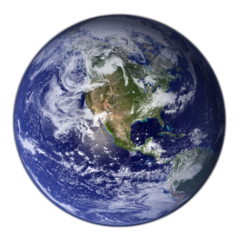
\includegraphics[width=1.8cm]{../../Figure/TBP/Earth.png}};
              % Text
              \node[below, shift={(0,-0.8)}] at (earth) {$m_1$};
              \node (a) at (A) {Earth};
              
              % Moon
              \node[circle, inner sep=5.5pt, fill=black!30] (MOON) at (moon) {};
              \node[inner sep=0pt] (moon_c) at (moon) {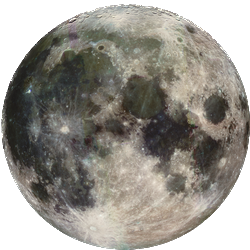
\includegraphics[width=.5cm]{../../Figure/TBP/Moon.png}};
              % Text 
              \node[below, shift={(0,-0.4)}] at (MOON) {$m_2$};
              \node (b) at (B) {Moon};
              
              % Lines
              \draw[-stealth] (a) to[bend left=30] ({\r*cos(\Phi)+1},{\r*sin(\Phi)+2});
              \draw[-stealth] (b) to[bend left=-30] (MOON);
              \draw[dashed, black] (earth) -- (MOON.center);
              
              % center of mass 0.25 from earth
              \coordinate (center) at ($(earth)!0.3!(MOON)$);
              % small circle
              \draw[fill=black] (center) circle (1.5pt) node[below, shift={(0,-0.1)}] {Center of Mass};
              
              % Calculate direction from Earth to Moon
              \pgfmathsetmacro{\xDiff}{8 - 1} % X difference between Moon and Earth
              \pgfmathsetmacro{\yDiff}{1 - 2} % Y difference between Moon and Earth
              \pgfmathsetmacro{\angle}{atan2(\yDiff,\xDiff)} % Angle of the line
              
              % Add axes at center of mass
              \draw[->, thick] (center) -- ++(\angle:2) node[above, shift={(0,0.2)}] {$x$ axis};
              \draw[->, thick] (center) -- ++(\angle+90:2) node[above] {$y$ axis};
              
              % add satellite with shift
              \coordinate (satellite) at ($(center)!0.5!(MOON)+(0,2)$);
              \node (satellite) at (satellite) {\faSatellite};
              
              % connect earth to satellite r1
              \draw[-stealth] (earth) -- (satellite) node[pos=0.3, above] {$\vb{r}_1$};   
              % connect moon to satellite r2
              \draw[-stealth] (MOON) -- (satellite) node[pos=0.5, above] {$\vb{r}_2$};
              % connect center of mass to satellite r
              \draw[-stealth] (center) -- (satellite) node[pos=0.5, above] {$\vb{r}$};
              % add line to show satellite is in between
              \node (c) at ($(satellite)+(1.5,0.5)$) {Satellite};
              \draw[-stealth] (c) to[bend left=30] (satellite);
            \end{tikzpicture}
          }
          \caption{CRTBP Configuration}
        \end{subfigure}%
        % \hfill
        % \hspace{-3.5cm}
        \begin{subfigure}{0.4\linewidth}
        %   \raggedleft
          \resizebox{\linewidth}{!}{%
        \begin{tikzpicture}
            % Define radius of the orbit
            \def\orbitRadius{4cm}
            
            % Draw the orbit circle with arrows
            \draw[-{Stealth[length=3mm]}, thick] (12:\orbitRadius) arc (12:170:\orbitRadius);
            \draw[-{Stealth[length=3mm]}, thick] (180:\orbitRadius) arc (180:355:\orbitRadius);
            
            % Position for Earth (center)
            \node[inner sep=0pt] (Earth) at (0,0) {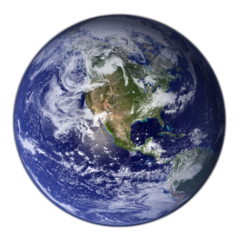
\includegraphics[width=1.8cm]{../../Figure/TBP/Earth.png}};
            \node[text=black] at (0,-1.3) {Earth};
            
            % Position for Moon (on the right side of the orbit)
            \node[inner sep=0pt] (Moon) at (0.95*\orbitRadius,0) {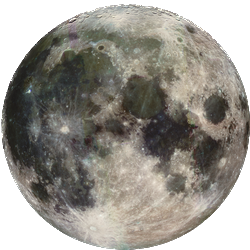
\includegraphics[width=0.6cm]{../../Figure/TBP/Moon.png}};
            \node[text=black] at (\orbitRadius,0.6) {Moon};
            
            % Lagrangian points
            \coordinate (L1) at (0.8*\orbitRadius,0);
            \coordinate (L2) at (1.2*\orbitRadius,0);
            \coordinate (L3) at (-1*\orbitRadius,0);
            \coordinate (L4) at (60:\orbitRadius);
            \coordinate (L5) at (300:\orbitRadius);
            
            % Draw Lagrangian points as red circles
            \foreach \point in {L1,L2,L3,L4,L5} {
                \fill[red] (\point) circle (0.1cm);
            }
            
            % Connect Lagrangian points with dashed lines
            \draw[dashed, blue, thick] (Earth) -- (L1);
            \draw[dashed, blue, thick] (Moon) -- (L1);
            \draw[dashed, blue, thick] (Moon) -- (L2);
            \draw[dashed, blue, thick] (Earth) -- (L3);
            \draw[dashed, blue, thick] (Earth) -- (L4);
            \draw[dashed, blue, thick] (Moon) -- (L4);
            \draw[dashed, blue, thick] (Earth) -- (L5);
            \draw[dashed, blue, thick] (Moon) -- (L5);
            
            % Labels for the Lagrangian points
            \node at ($(L1) + (0,0.5)$) {$L_1$};
            \node at ($(L2) + (0,0.5)$) {$L_2$};
            \node at ($(L3) + (0,0.5)$) {$L_3$};
            \node at ($(L4) + (0.5,0.3)$) {$L_4$};
            \node at ($(L5) + (0.5,-0.3)$) {$L_5$};
        \end{tikzpicture}
          }
        %   \raggedright
          \caption{Lagrangian points in the Earth-Moon system}
        \end{subfigure}
        \vspace{-0.2cm}
        \caption{CRTBP Model and Lagrangian Points}
  \end{figure}
\end{frame}
%           \draw[-stealth] (center) -- (satellite) node[pos=0.5, above] {$\vb{r}$};
%           % add line to show satellite is in between
%           \node (c) at ($(satellite)+(1.5,0.5)$) {Satellite};
%           \draw[-stealth] (c) to[bend left=30] (satellite);
%         \end{tikzpicture}
%       }
%       \caption{CRTBP Configuration}
%     \end{subfigure}
%     \caption{Duplicated CRTBP geometric schematic (side-by-side).}
%   \end{figure}
% \end{frame}


% --- Appendix (keeps parameter + RL/MARL theoretical extras if any later) ---
\appendix

% (optional future) \section{RL Algorithm Parameters}

\begin{frame}
  \frametitle{DDPG Parameters}
  \scriptsize
  \begin{tabular}{|l|c||l|c|}
  \hline
  Steps / epoch & 30k & Epochs & 100 \\ \hline
  Buffer size & $10^{6}$ & Discount $\gamma$ & 0.99 \\ \hline
  Polyak $\tau$ & 0.995 & Actor LR & $1\!\times\!10^{-3}$ \\ \hline
  Critic LR & $1\!\times\!10^{-3}$ & Batch size & 1024 \\ \hline
  Start policy steps & 5k & Update start & 1k \\ \hline
  Update interval & 2k & Action noise & 0.1 \\ \hline
  Max episode len & 6k & Device & Cuda \\ \hline
  Net (A/C) & (32,32) & Act fn & ReLU \\ \hline
  \end{tabular}
\end{frame}

\begin{frame}
  \frametitle{TD3 Parameters}
  \scriptsize
  \begin{tabular}{|l|c||l|c|}
  \hline
  Steps / epoch & 30k & Epochs & 100 \\ \hline
  Buffer size & $10^{6}$ & Discount $\gamma$ & 0.99 \\ \hline
  Polyak $\tau$ & 0.995 & Actor LR & $1\!\times\!10^{-3}$ \\ \hline
  Critic LR & $1\!\times\!10^{-3}$ & Batch size & 1024 \\ \hline
  Start policy steps & 5k & Update start & 1k \\ \hline
  Update interval & 2k & Target noise & 0.2 \\ \hline
  Noise clip & 0.5 & Policy delay & 2 \\ \hline
  Max episode len & 30k & Nets (A/C) & (32,32) \\ \hline
  \end{tabular}
\end{frame}

\begin{frame}
  \frametitle{SAC Parameters}
  \scriptsize
  \begin{tabular}{|l|c||l|c|}
  \hline
  Steps / epoch & 30k & Epochs & 100 \\ \hline
  Buffer size & $10^{6}$ & Discount $\gamma$ & 0.99 \\ \hline
  Polyak $\tau$ & 0.995 & LR (all) & $1\!\times\!10^{-3}$ \\ \hline
  Alpha init & 0.2 & Batch size & 1024 \\ \hline
  Start steps & 5k & Update start & 1k \\ \hline
  Updates / step & 10 & Update interval & 2k \\ \hline
  Test episodes & 10 & Max len & 30k \\ \hline
  Nets (A/C) & (32,32) & Activation & ReLU \\ \hline
  \end{tabular}
\end{frame}

\begin{frame}
  \frametitle{PPO Parameters}
  \scriptsize
  \begin{tabular}{|l|c||l|c|}
  \hline
  Steps / epoch & 30k & Epochs & 100 \\ \hline
  Discount $\gamma$ & 0.99 & Clip ratio & 0.2 \\ \hline
  Policy LR & $3\!\times\!10^{-4}$ & Value LR & $1\!\times\!10^{-3}$ \\ \hline
  Policy iters & 80 & Value iters & 80 \\ \hline
  Nets (Actor) & (32,32) & Nets (Critic) & (32,32) \\ \hline
  Activation & ReLU & Batch (mini) & (derived) \\ \hline
  \end{tabular}
\end{frame}

\begin{frame}
  \frametitle{Training Procedure (Summary)}
  \small
  \begin{enumerate}\setlength{\itemsep}{2pt}
    \item Collect initial random experience (fill replay / buffer).
    \item Loop: act, store $(s,a,r,s',d)$, update (per algo rules).
    \item Target networks: Polyak averaging ($\tau$).
    \item TD3: twin critics + delayed policy + target smoothing.
    \item SAC: entropy term, adaptive temperature (if enabled).
    \item PPO: clipped surrogate objective, on-policy batches.
    \item Stability: normalization, gradient clipping (if needed), fixed seeds.
  \end{enumerate}
\end{frame}



\end{document}
% %------------------------------------------------
% \begin{frame}
% 	\frametitle{Research Motivation}
	
% 	\begin{itemize}
% 		\item \textbf{Space missions} increasingly require autonomous guidance systems
% 		\item \textbf{Low-thrust spacecraft} operate in complex gravitational environments
% 		\item \textbf{Three-body dynamics} (Earth-Moon CRTBP) present inherent instabilities
% 		\item \textbf{Classical control methods} struggle with:
% 		\begin{itemize}
% 			\item Model uncertainties
% 			\item Environmental disturbances
% 			\item Fuel efficiency requirements
% 		\end{itemize}
% 		\item \textbf{Need for robust, adaptive guidance} without precise dynamic models
% 	\end{itemize}
	
% 	\vspace{0.3cm}
% 	\begin{center}
% 		\textit{How can we achieve robust spacecraft guidance in uncertain environments?}
% 	\end{center}
% \end{frame}

% %------------------------------------------------
% \begin{frame}
% 	\frametitle{Problem Statement}
%     \vspace{-0.35cm}
% 	\begin{block}{Research Objective}
% 		Design a robust guidance framework for low-thrust spacecraft operating in Earth-Moon three-body dynamics under uncertainties.
% 	\end{block}
	
% 	\begin{columns}[t]
% 		\begin{column}{0.5\textwidth}
% 			\textbf{System Characteristics:}
% 			\begin{itemize}
% 				\item State: $\mathbf{x} = [x, y, \dot{x}, \dot{y}]^T$
% 				\item Control: $\mathbf{u} \leq u_{\max}$
% 				\item Dynamics: $\dot{\mathbf{x}} = f(\mathbf{x}, \mathbf{u})$
% 			\end{itemize}
% 		\end{column}
% 		\begin{column}{0.5\textwidth}
% 			\textbf{Mission Environment:}
% 			\begin{itemize}
% 				\item Earth-Moon CRTBP
% 				\item Lyapunov orbit transfer
% 				\item Low-thrust propulsion
% 				% \item Real-time constraints
% 			\end{itemize}
% 		\end{column}
% 	\end{columns}
	
% 	% \vspace{-0.}
%     \begin{minipage}
%         {0.93\textwidth}
%             \begin{exampleblock}{Mathematical Formulation}
% 		Optimal control problem with state-dependent uncertainties and adversarial disturbances
% 	\end{exampleblock}
%     \end{minipage}
% \end{frame}

% %------------------------------------------------
% \begin{frame}
%     \frametitle{Problem Statement - Challenges \& Approach}
    
%     \begin{columns}[T,onlytextwidth]
%         \begin{column}{0.45\textwidth}
%             \textbf{Uncertainty Sources:}
%             \begin{itemize}
%                 \item Random initial conditions
%                 \item Actuator disturbances
%                 \item Sensor noise
%                 \item Model mismatch
%                 \item Communication delays
%                 \item External perturbations
%             \end{itemize}
%         \end{column}
%         \begin{column}{0.55\textwidth}
%             \textbf{Design Requirements:}
%             \begin{itemize}
%                 \item Robust performance
%                 \item Fuel efficiency
%                 \item Real-time capability
%                 \item Model-free approach
%                 \item Adaptive behavior
%                 \item Safety guarantees
%             \end{itemize}
%         \end{column}
%     \end{columns}
    
%     \vspace{-0.1cm}
%     \begin{minipage}
%         {0.93\textwidth}
%             \begin{alertblock}{Key Challenge}
%         Formulate as zero-sum differential game: spacecraft vs. environmental disturbances
%     \end{alertblock}
%     \end{minipage} 

% \end{frame}

    
% %------------------------------------------------
% \section{Methodology}

% %------------------------------------------------
% \begin{frame}
% 	\frametitle{Multi-Agent Reinforcement Learning Framework}
	
% 	\begin{columns}[t]
% 		\begin{column}{0.6\textwidth}
% 			\textbf{Game-Theoretic Formulation:}
% 			\begin{itemize}
% 				\item \textbf{Player 1}: Controller agent (spacecraft)
% 				\item \textbf{Player 2}: Adversary agent (disturbances)
% 				\item \textbf{Objective}: Zero-sum differential game
% 			\end{itemize}
			
% 			\vspace{0.3cm}
% 			\textbf{Training Paradigm:}
% 			\begin{itemize}
% 				\item Centralized training
% 				\item Decentralized execution
% 				% \item Shared actor-critic networks
% 			\end{itemize}
% 		\end{column}
% 		\begin{column}{0.4\textwidth}
% 			\begin{figure}
% 				\centering
% 				
\includegraphics[width=\textwidth]{framework_diagram.png}
% 				\caption{MARL Framework}
% 			\end{figure}
% 		\end{column}
% 	\end{columns}
	
% 	\begin{exampleblock}{Innovation}
% 		Extension of single-agent RL algorithms (DDPG, TD3, SAC, PPO) to multi-agent zero-sum variants (MA-DDPG, MATD3, MASAC, MAPPO)
% 	\end{exampleblock}
% \end{frame}

% %------------------------------------------------
% \begin{frame}
% 	\frametitle{Algorithm Extensions}
	
% 	\begin{block}{Single-Agent $\rightarrow$ Multi-Agent Zero-Sum}
% 		Extended four continuous RL algorithms to handle adversarial scenarios
% 	\end{block}
	
% 	\begin{columns}[t]
% 		\begin{column}{0.5\textwidth}
% 			\textbf{DDPG $\rightarrow$ MA-DDPG}
% 			\begin{itemize}
% 				\item Deterministic policy gradient
% 				\item Experience replay
% 				\item Target networks
% 			\end{itemize}
			
% 			% \vspace{0.1cm}
% 			\textbf{SAC $\rightarrow$ MA-SAC}
% 			\begin{itemize}
% 				\item Entropy regularization
% 				\item Stochastic policies
% 				\item Automatic temperature tuning
% 			\end{itemize}
% 		\end{column}
% 		\begin{column}{0.5\textwidth}
% 			\textbf{TD3 $\rightarrow$ MA-TD3}
% 			\begin{itemize}
% 				\item Twin critic networks
% 				\item Delayed policy updates
% 				\item Target policy smoothing
% 			\end{itemize}
			
% 			% \vspace{0.1cm}
% 			\textbf{PPO $\rightarrow$ MA-PPO}
% 			\begin{itemize}
% 				\item Proximal policy optimization
% 				\item Clipped surrogate objective
% 				\item On-policy learning
% 			\end{itemize}
% 		\end{column}
% 	\end{columns}
% \end{frame}

% %------------------------------------------------
% \begin{frame}
% 	\frametitle{Network Architecture}
	
% 	\begin{columns}[t]
% 		\begin{column}{0.5\textwidth}
% 			\textbf{Actor-Critic Structure:}
% 			\begin{itemize}
% 				\item 3 hidden layers
% 				\item 32 neurons per layer
% 				\item ReLU activation
% 				\item Learning rate: $3 \times 10^{-4}$
% 			\end{itemize}
			
% 			\vspace{0.3cm}
% 			\textbf{Training Parameters:}
% 			\begin{itemize}
% 				\item 1M environment steps
% 				\item Batch size: 1024
% 				\item Buffer size: 100K
% 				\item Adam optimizer
% 			\end{itemize}
% 		\end{column}
% 		\begin{column}{0.5\textwidth}
% 			\begin{figure}
% 				\centering
% 				
\includegraphics[width=\textwidth]{network_architecture.png}
% 				\caption{Network Structure}
% 			\end{figure}
% 		\end{column}
% 	\end{columns}
	
% 	\begin{block}{Shared Networks}
% 		Both agents use identical network architectures with separate parameter sets for competitive learning
% 	\end{block}
% \end{frame}

% %------------------------------------------------
% \section{Experimental Setup}

% %------------------------------------------------
% \begin{frame}
% 	\frametitle{Evaluation Scenarios}
	
% 	\begin{block}{Mission: Transfer to Earth-Moon Lyapunov Orbit}
% 		Circular Restricted Three-Body Problem (CRTBP) environment
% 	\end{block}
	
% 	\begin{columns}[t]
% 		\begin{column}{0.5\textwidth}
% 			\textbf{Uncertainty Scenarios:}
% 			\begin{enumerate}
% 				\item Random initial states ($\sigma = 0.1$)
% 				\item Actuator disturbances ($\sigma = 0.05$)
% 				\item Model mismatch ($\sigma = 0.05$)
% 				\item Partial observations (50\% missing)
% 				\item Sensor noise ($\sigma = 0.05$)
% 				\item Communication delays (10 steps)
% 			\end{enumerate}
% 		\end{column}
% 		\begin{column}{0.5\textwidth}
% 			\textbf{Performance Metrics:}
% 			\begin{itemize}
% 				\item Trajectory accuracy
% 				\item Fuel consumption
% 				\item System stability
% 				\item Convergence rate
% 				\item Robustness measures
% 			\end{itemize}
			
% 			% \vspace{0.3cm}
% 			\textbf{Baseline Comparison:}
% 			\begin{itemize}
% 				\item Single-agent variants
% 				% \item Classical LQR/LQG
% 				% \item Model predictive control
% 			\end{itemize}
% 		\end{column}
% 	\end{columns}
% \end{frame}

% %------------------------------------------------
% \section{Results}

% %------------------------------------------------
% \begin{frame}
% 	\frametitle{Trajectory Comparison: MA-TD3 Performance}
% 	\vspace{-.75cm}
% 	\begin{columns}[t]
% 		\begin{column}{0.5\textwidth}
% 			\begin{figure}
% 				\centering
% 				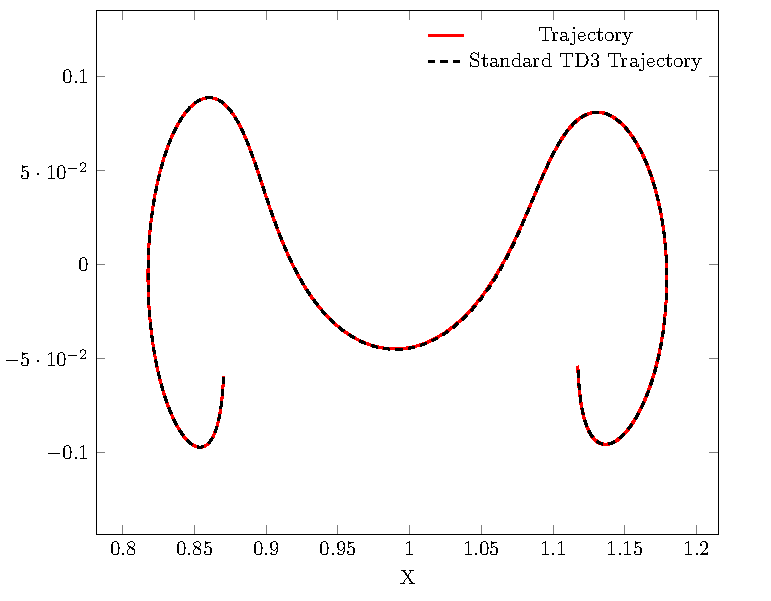
\includegraphics[width=.7\textwidth]{../../Report/plots/td3/trajectory_force/plot_trajectory}
% 				\vspace{-.5cm}
% 				\caption{Single-Agent vs Multi-Agent TD3}
% 			\end{figure}
% 		\end{column}
% 		\begin{column}{0.5\textwidth}
% 			\begin{figure}
% 				\centering
% 				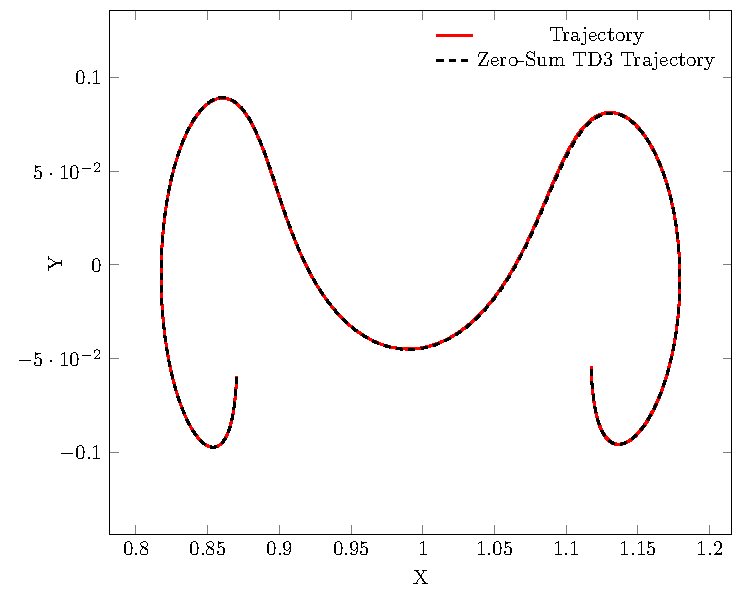
\includegraphics[width=.7\textwidth]{../../Report/plots/td3/trajectory_force/plot_trajectory_zs}
% 				\vspace{-.5cm}
% 				\caption{Thrust Commands}
% 			\end{figure}
% 		\end{column}
% 	\end{columns}
% 	\vspace{-0.5cm}
% 	\begin{alertblock}{Key Observation}
% 		Zero-sum variants demonstrate more direct trajectories with smoother thrust profiles and reduced fuel consumption
% 	\end{alertblock}
% \end{frame}

% %------------------------------------------------
% \begin{frame}
% 	\frametitle{Robustness Evaluation Results}
	
% 	\begin{figure}
% 		\centering
% 		
\includegraphics[width=0.9\textwidth]{robustness_comparison_all.png}
% 		\caption{Performance under different uncertainty scenarios}
% 	\end{figure}
	
% 	\begin{block}{Key Findings}
% 		\begin{itemize}
% 			\item Zero-sum variants consistently outperform single-agent baselines
% 			\item MATD3 shows best overall performance across all scenarios
% 			\item Significant improvements in sensor noise and time delay scenarios
% 		\end{itemize}
% 	\end{block}
% \end{frame}

% %------------------------------------------------
% \begin{frame}
% 	\frametitle{Algorithm Performance Comparison}
	
% 	\begin{columns}[t]
% 		\begin{column}{0.5\textwidth}
% 			\textbf{Single-Agent Algorithms:}
% 			\begin{figure}
% 				\centering
% 				
\includegraphics[width=\textwidth]{single_agent_comparison.png}
% 				\caption{Standard RL Performance}
% 			\end{figure}
% 		\end{column}
% 		\begin{column}{0.5\textwidth}
% 			\textbf{Multi-Agent Zero-Sum:}
% 			\begin{figure}
% 				\centering
% 				
\includegraphics[width=\textwidth]{multi_agent_comparison.png}
% 				\caption{Zero-Sum RL Performance}
% 			\end{figure}
% 		\end{column}
% 	\end{columns}
	
% 	\begin{exampleblock}{Best Performer}
% 		MATD3 achieves optimal trade-off between trajectory accuracy and propellant consumption while maintaining stability in harsh conditions
% 	\end{exampleblock}
% \end{frame}

% %------------------------------------------------


% %------------------------------------------------
% \section{Contributions \& Conclusions}

% %------------------------------------------------
% \begin{frame}
% 	\frametitle{Research Contributions}
	
% 	\begin{enumerate}
% 		\item \textbf{Novel Framework Development}
% 		\begin{itemize}
% 			\item First multi-agent zero-sum RL framework for spacecraft guidance in CRTBP
% 			\item Game-theoretic formulation for robust control under uncertainties
% 		\end{itemize}
		
% 		\item \textbf{Algorithm Extensions}
% 		\begin{itemize}
% 			\item Extended four major RL algorithms to multi-agent zero-sum variants
% 			\item Comprehensive performance analysis across uncertainty scenarios
% 		\end{itemize}
		
% 		\item \textbf{Practical Implementation}
% 		\begin{itemize}
% 			\item Real-time deployment with quantization and optimization
% 			\item Hardware-in-the-loop validation on ROS 2 platform
% 		\end{itemize}
		
% 		\item \textbf{Performance Validation}
% 		\begin{itemize}
% 			\item Demonstrated superior robustness compared to classical methods
% 			\item Quantified improvements in fuel efficiency and trajectory accuracy
% 		\end{itemize}
% 	\end{enumerate}
% \end{frame}

% %------------------------------------------------
% \begin{frame}
% 	\frametitle{Conclusions}
	
% 	\begin{block}{Main Findings}
% 		\begin{itemize}
% 			\item Multi-agent zero-sum RL enables robust spacecraft guidance without precise dynamic models
% 			\item MATD3 delivers optimal performance across all evaluation scenarios
% 			\item Framework is ready for practical deployment with real-time constraints
% 		\end{itemize}
% 	\end{block}
	
% 	\begin{columns}[t]
% 		\begin{column}{0.5\textwidth}
% 			\textbf{Advantages:}
% 			\begin{itemize}
% 				\item Model-free approach
% 				\item Adaptive to uncertainties
% 				\item Fuel-efficient trajectories
% 				\item Real-time capability
% 			\end{itemize}
% 		\end{column}
% 		\begin{column}{0.5\textwidth}
% 			\textbf{Future Work:}
% 			\begin{itemize}
% 				\item 3D CRTBP extension
% 				\item Multi-body dynamics
% 				\item Swarm coordination
% 				\item Deep space missions
% 			\end{itemize}
% 		\end{column}
% 	\end{columns}
	
% 	\vspace{0.3cm}
% 	\begin{center}
% 		\textbf{The framework opens new possibilities for autonomous space exploration}
% 	\end{center}
% \end{frame}

% %---------------------------------------------------------
% %	CLOSING SLIDE
% %---------------------------------------------------------

% % To remove miniframe from top
% \appendix
% \setbeamertemplate{headline}{}
% \addtobeamertemplate{frametitle}{\vspace*{-\headheight}}{}

% \begin{frame}[noframenumbering]
% 	\begin{center}
% 		{\LARGE Thank You!}
		
% 		\vspace{1cm}
		
% 		{\large Questions \& Discussion}
		
% 		\vspace{1cm}
		
% 			\textit{Ali Baniasad} 
% 			% extit{alibaniasad1999@gmail.com} 
		
% 		\vspace{0.5cm}
		
% 		Department of Aerospace Engineering \\ 
% 		Sharif University of Technology
% 	\end{center}
% \end{frame}

% %---------------------------------------------------------
% %	APPENDIX SLIDES
% %---------------------------------------------------------

% %------------------------------------------------
% \begin{frame}[noframenumbering]
% \label{Technical Details}
% 	\frametitle{Appendix - Technical Implementation Details}
	
% 	\begin{columns}[t]
% 		\begin{column}{0.5	extwidth}
% 				extbf{Environment Setup:}
% 			\begin{itemize}
% 				\item PyTorch \& OpenAI Gym
% 				\item CRTBP dynamics implementation
% 				\item Custom reward function design
% 				\item Parallel environment execution
% 			\end{itemize}
			
% 			\vspace{0.3cm}
			
% 				extbf{Network Architecture:}
% 			\begin{itemize}
% 				\item Input: 4D state vector
% 				\item Hidden: 3 layers × 256 neurons
% 				\item Output: 2D action vector (thrust)
% 				\item Activation: ReLU
% 			\end{itemize}
% 		\end{column}
% 		\begin{column}{0.5	extwidth}
% 				extbf{Training Configuration:}
% 			\begin{itemize}
% 				\item Episodes: 1M steps
% 				\item Batch size: 1024
% 				\item Learning rate: 3e-4
% 				\item Discount factor: 0.99
% 				\item Replay buffer: 100K
% 			\end{itemize}
			
% 			\vspace{0.3cm}
			
% 				extbf{Evaluation Metrics:}
% 			\begin{itemize}
% 				\item Cumulative reward
% 				\item Trajectory deviation
% 				\item Fuel consumption
% 				\item Convergence stability
% 			\end{itemize}
% 		\end{column}
% 	\end{columns}
% \end{frame}

% %------------------------------------------------
% \begin{frame}[noframenumbering]
% \label{Algorithm Details}
% 	\frametitle{Appendix - Zero-Sum Algorithm Extensions}
	
% 	\begin{block}{MATD3 Algorithm Highlights}
% 		\begin{itemize}
% 			\item Twin critic networks to reduce overestimation bias
% 			\item Delayed policy updates for stability
% 			\item Target policy smoothing for robustness
% 			\item Competitive training between agents
% 		\end{itemize}
% 	\end{block}
	
% 	\begin{columns}[t]
% 		\begin{column}{0.5	extwidth}
% 				extbf{Key Modifications:}
% 			\begin{enumerate}
% 				\item Shared environment state
% 				\item Adversarial action selection
% 				\item Minimax objective function
% 				\item Nash equilibrium convergence
% 			\end{enumerate}
% 		\end{column}
% 		\begin{column}{0.5	extwidth}
% 				extbf{Performance Benefits:}
% 			\begin{enumerate}
% 				\item Enhanced robustness
% 				\item Better generalization
% 				\item Improved worst-case handling
% 				\item Stable learning dynamics
% 			\end{enumerate}
% 		\end{column}
% 	\end{columns}
% \end{frame}

% %------------------------------------------------
% \begin{frame}[noframenumbering]
% \label{Future Work}
% 	\frametitle{Appendix - Future Research Directions}
	
% 	\begin{enumerate}
% 		\item 	extbf{Multi-Body Extensions}
% 		\begin{itemize}
% 			\item Sun-Earth-Moon system
% 			\item Jupiter-Europa dynamics
% 			\item Asteroid belt navigation
% 		\end{itemize}
		
% 		\item 	extbf{Swarm Coordination}
% 		\begin{itemize}
% 			\item Formation flying control
% 			\item Distributed decision making
% 			\item Communication constraints
% 		\end{itemize}
		
% 		\item 	extbf{Advanced Techniques}
% 		\begin{itemize}
% 			\item Meta-learning approaches
% 			\item Hierarchical reinforcement learning
% 			\item Physics-informed neural networks
% 		\end{itemize}
		
% 		\item 	extbf{Mission Applications}
% 		\begin{itemize}
% 			\item Lunar gateway operations
% 			\item Deep space exploration
% 			\item Interplanetary transfers
% 		\end{itemize}
% 	\end{enumerate}
% \end{frame}

% %------------------------------------------------
% \begin{frame}[noframenumbering]
% \label{Figure}
% 	\frametitle{Appendix - A figure}
%         \hyperlink{Test}{\beamerreturnbutton{Return to presentation}}

%         \begin{figure}[h!]
%             \centering
%             %\caption{}
%             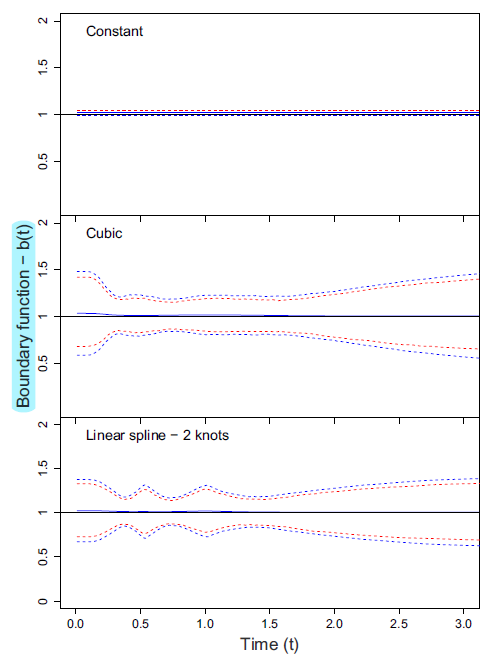
\includegraphics[angle=0, width=5cm]{Newey et al Graph.png}
%             %\label{fig}
%         \end{figure}
% \end{frame}

% %------------------------------------------------
% \begin{frame}[noframenumbering]
% \label{Terms}
% 	\frametitle{Appendix - Terms}

%         \begin{columns}[t] % The "c" option specifies centered vertical alignment while the "t" option is used for top vertical alignment
% 		\begin{column}{0.5\textwidth} % Right column width
%                 Some Estimators:
%                 \begin{itemize}
%                     \item Drift: $\hat{\delta}$
%                     \item Boundary: $\hat{b}(t)$
%                 \end{itemize}
% 		\end{column}
%   		\begin{column}{0.5\textwidth} % Left column width
%                 Some Variables:
%                 \begin{itemize}
%                     \item $\hat{V}$
%                     \item $\hat{m}_S$
%                     \item $\bar{m}$
%                     \item $m_J(\tau)$\newline\newline
%                 \end{itemize}
% 		\end{column}
% 	\end{columns}
%         \hyperlink{Test Stat}{\beamerreturnbutton{Return to presentation}}
% \end{frame}

% %------------------------------------------------
% \begin{frame}[noframenumbering]
% \label{Definitions}
% 	\frametitle{Appendix - Definitions}
%          \begin{enumerate}
%              \item A definition \newline
%          \end{enumerate}

%         \hyperlink{Test Stat}{\beamerreturnbutton{Return to presentation}}
% \end{frame}

% %------------------------------------------------
% \begin{frame}[noframenumbering]
% \label{Theorems}
% 	\frametitle{Appendix - Theorems}
%          \begin{enumerate}
%              \item A theorem\newline
%          \end{enumerate}

%         \hyperlink{Test Stat}{\beamerreturnbutton{Return to presentation}}
% \end{frame}

\end{document}
\end{document}
